\section{Locality Sensitive Hashing}\label{sec:hashing}

The embedding defined by our joint network architecture is a high dimensional space. Taking the last fully-connected layer of the tuple branches to be the embedding for a tuple gives a point in a 128 dimensional space. The naive retrieval algorithm would then project all videos in the database into this space, then for each probe, project it into the same space and execute a nearest neighbor search. The search would return video ranked by their $l_2$ distance in the 128 dimensional space.

Generally, this is a slow computation. Note that for a single comparison, 

\begin{equation}
    d(x, y) = \sqrt{\sum_{i=0}^{128} (x_i - y_i)^2}
\end{equation} 
Being optimistic and ignoring the square root, this requires 256 additions and 128 multiplies per video in the database, after which $N$ comparisons must be made for a database of size $N$. This does not scale well to large databases.

There are several potential solutions to this which all reduce to a dimensionality reduction. We choose a highly efficient method: Locality Sensitive Hashing (LSH). Most hash functions, such as those used in cryptography or for $O(1)$ storage mechanisms, try to distribute their results evenly in the output space. For example, a cryptographically secure hash should result in a distribution of the output bits that appears random to an observer with no knowledge of the input. For a LSH, the goal is the opposite. Inputs should preserve the ordering of their distances when projected into the hashed space. Formally, given three points in some space $x_0, x_1, x_2$ such that 

\begin{equation}
|x_0 - x_1|_2 > |x_0 - x_2|_2
\end{equation}
we desire

\begin{equation}
|H(x_0) - H(x_1)|_2 > |H(x_0) - H(x_2)|_2
\end{equation}

We choose the Random Projects, or SimHash \cite{charikar2002similarity}, algorithm for this purpose. The Random Projections algorithm defines $k$ random hyperplanes in the space of the original points. For each point $x$, the hash function $H(x)$ computes

\begin{align}
    p_i = \text{sign}(k_i \cdot x) \\
    H(x) = p_0...p_k
\end{align}

Such that each of the $p_i$ are encoded as a single bit. In this way, the function $H(x)$ defines a $k$-bit Hamming space \cite{hamming1950error}. The $k$ hyperplanes should be uniformly distributed in the input space. Using this algorithm allows us to use the Hamming distance function, which is extremely fast to compute using bitwise operations \cite{cohen1997covering}.

\begin{figure}[h]
    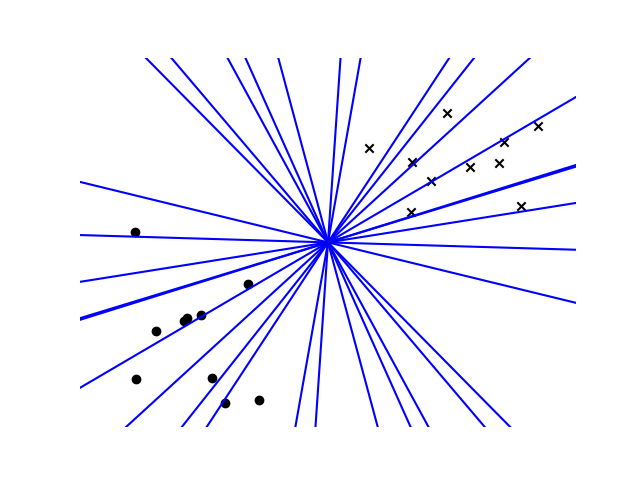
\includegraphics[width=0.5\textwidth]{images/lsh_planes.png}
    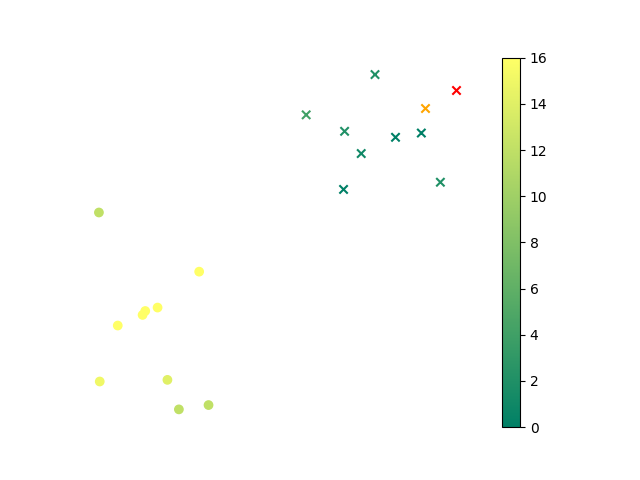
\includegraphics[width=0.5\textwidth]{images/lsh_distance.png}
    \caption{Top: Hyperplanes and points in 2D space, Bottom: Hamming distance from red point to all other points. Nearest neighbor in hamming space is highlighted in orange.}
    \label{fig:lsh}
\end{figure}

The number of hyperplanes $k$ is a tunable parameter. In general, a higher $k$ gives more accurate distances for a slower distance computation. Figure \ref{fig:lsh} Top shows a set of 16 hyperplanes that could be used to encode the set of 2D points. Figure 1 Bottom ranks the points based on their distance from the red point, with the nearest neighbor in hamming space highlighted in orange. Examining Figure \ref{fig:lsh} Top gives some intuition about why the Random Projections algorithm works: as the number of planes goes to infinity, the distance metric approaches the cosine distance between the points. This intuitive result is proven by Charikar \cite{charikar2002similarity}.

